% 2020 天津卷 第 15 题：四边形 ABCD 与线段 BC 上的动点 M、N
% 来源 PDF：普通高考/2020/2020天津.pdf 第 1 页（A3 横排），印面 1131，第 15 题题干下方
% 几何按原页矢量数据换算（原页 1 个长度单位 ≈ 19.83 pt）：
%   B=(0,0)，C=(6,0)（BC=6），∠B=60°、AB=3 给出 A=(1.5, 3√3/2)，
%   AD=λ·BC 且 AD∥BC，λ=1/6 给出 D=(1.5+1, 3√3/2)=(2.5, 3√3/2)；
%   坐标为真实长度（1 单位 = BC 的六分之一），故 M=(3.4,0)、N=(4.4,0) 已满足 |MN|=1，
%   且与原页 M、N 的位置一致。原页只连 DM、DN 两条线段，未连其他辅助线。
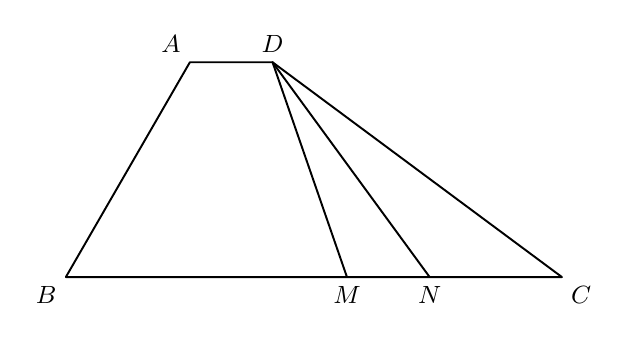
\begin{tikzpicture}[font=\small, line width=0.7pt,
  x=1.05cm, y=1.05cm, line cap=round, line join=round]
  \coordinate (B) at (0,0);
  \coordinate (C) at (6,0);
  \coordinate (A) at (1.5,2.598);
  \coordinate (D) at (2.5,2.598);
  \coordinate (M) at (3.4,0);
  \coordinate (N) at (4.4,0);
  \draw (B)--(C)--(D)--(A)--cycle;
  \draw (D)--(M);
  \draw (D)--(N);
  \node[below left,inner sep=3pt] at (B) {$B$};
  \node[below right,inner sep=3pt] at (C) {$C$};
  \node[above left,inner sep=3pt] at (A) {$A$};
  \node[above,inner sep=3pt] at (D) {$D$};
  \node[below,inner sep=3pt] at (M) {$M$};
  \node[below,inner sep=3pt] at (N) {$N$};
\end{tikzpicture}
